\section{Theory}
\label{app:theory}

\subsection{One-Reset Error Propagation}
\label{app:one-reset-error}

This section formalizes the error-propagation challenge under a one-reset simplification. For clarity, we analyze the conditional mean of the target representation and omit process noise. The stochastic case follows by adding the corresponding covariance terms to the Gaussian energy.

Recall the switched affine representation dynamics
\begin{equation}
    \psi_{t+1}
    =
    A_{\omega_t}\psi_t
    +
    \omega_t b_t,
\end{equation}
where $\omega_t=0$ denotes passive target dynamics and $\omega_t=1$ denotes an interaction. Let
\begin{equation}
    \tau
    =
    \inf\{\ell\ge 0:\omega_{t+\ell}=1\}
\end{equation}
be the first future interaction offset after anchor $x_t$. In the one-reset case, the mode sequence has the form
\[
    0,0,\ldots,0,1,0,\ldots,0.
\]
That is, the target evolves passively before the interaction, experiences one interaction reset, and then evolves passively again.

\subsection{One-Reset Future Mean}

Before the interaction, the target representation follows passive dynamics:
\begin{equation}
    \psi_{t+\tau}
    =
    A_0^\tau \psi_t .
\end{equation}
At the interaction step,
\begin{equation}
    \psi_{t+\tau+1}
    =
    A_1\psi_{t+\tau}
    +
    b_{t+\tau}.
\end{equation}
Define the bridge shift
\begin{equation}
    \delta_{\tau}
    =
    (A_1-A_0)\psi_{t+\tau}
    +
    b_{t+\tau}.
    \label{eq:bridge-shift-appendix}
\end{equation}
Then the interaction update can be written as a passive update plus a bridge shift:
\begin{equation}
    \psi_{t+\tau+1}
    =
    A_0\psi_{t+\tau}
    +
    \delta_{\tau}.
\end{equation}

Now consider a future sampled $k$ passive steps after the interaction. Equivalently, the total horizon is
\[
    n=\tau+1+k.
\]
Then
\begin{equation}
    \psi_{t+n}
    =
    A_0^k
    \left(
    A_0\psi_{t+\tau}
    +
    \delta_{\tau}
    \right).
\end{equation}
Substituting $\psi_{t+\tau}=A_0^\tau\psi_t$ gives
\begin{equation}
    \psi_{t+n}
    =
    A_0^{\tau+1+k}\psi_t
    +
    A_0^k\delta_{\tau}.
    \label{eq:one-reset-future-mean}
\end{equation}

Thus, the bridge shift is observed directly only when $k=0$. For later futures, the bridge shift is observed through the propagated term $A_0^k\delta_{\tau}$.

\subsection{Mixture over Reset Times}

For a fixed horizon $n$, the reset time may be latent. If the interaction occurs at offset $\ell$, then $k=n-\ell-1$, and the corresponding future mean is
\begin{equation}
    \mu_n^{(\ell)}
    =
    A_0^n\psi_t
    +
    A_0^{n-\ell-1}\delta_{\ell},
    \qquad
    \delta_{\ell}
    =
    (A_1-A_0)\psi_{t+\ell}
    +
    b_{t+\ell}.
\end{equation}
Therefore, even in the one-reset case, the future distribution is a mixture over possible reset times:
\begin{equation}
    p(\psi_{t+n}\mid x_t)
    =
    \sum_{\ell=0}^{n-1}
    p(\tau=\ell\mid x_t)
    \,
    \mathcal N
    \left(
    \mu_n^{(\ell)},
    \Sigma_{\ell}
    \right).
    \label{eq:one-reset-mixture}
\end{equation}

\subsection{Representation Error from Bridge Error}

We now analyze how an error in estimating the bridge shift affects the endpoint future representation.

\begin{lemma}[Propagated bridge error]
\label{lem:propagated-bridge-error}
Suppose the true bridge shift is $\delta_{\tau}$ and the learned bridge shift is
\begin{equation}
    \widehat{\delta}_{\tau}
    =
    \delta_{\tau}
    +
    e_{\tau}.
\end{equation}
For a future sampled $k$ passive steps after the interaction, the induced future-mean error is
\begin{equation}
    \widehat{\mu}_k-\mu_k
    =
    A_0^k e_{\tau}.
    \label{eq:future-mean-error}
\end{equation}
Consequently,
\begin{equation}
    \|\widehat{\mu}_k-\mu_k\|
    \le
    \|A_0^k\|
    \|e_{\tau}\|.
    \label{eq:future-mean-error-bound}
\end{equation}
\end{lemma}

\begin{proof}
From Eq.~\eqref{eq:one-reset-future-mean}, the true future mean is
\begin{equation}
    \mu_k
    =
    A_0^{\tau+1+k}\psi_t
    +
    A_0^k\delta_{\tau}.
\end{equation}
Using the learned bridge shift gives
\begin{equation}
    \widehat{\mu}_k
    =
    A_0^{\tau+1+k}\psi_t
    +
    A_0^k\widehat{\delta}_{\tau}.
\end{equation}
Subtracting the two expressions yields
\begin{equation}
    \widehat{\mu}_k-\mu_k
    =
    A_0^k
    \left(
    \widehat{\delta}_{\tau}
    -
    \delta_{\tau}
    \right)
    =
    A_0^k e_{\tau}.
\end{equation}
The norm bound follows from submultiplicativity of the operator norm.
\end{proof}

Lemma~\ref{lem:propagated-bridge-error} shows that the endpoint representation error is not only determined by the local bridge error $e_{\tau}$, but also by the post-interaction propagation factor $A_0^k$.

\subsection{Energy Error from Bridge Error}

We next translate this propagated representation error into an energy error. Let
\[
    z_f=\psi(y_f)
\]
be the sampled future representation. Under the local Gaussian approximation, the energy assigned to $z_f$ is
\begin{equation}
    E_k(x_t,y_f)
    =
    -\frac{1}{2}
    \|z_f-\mu_k\|_{\Sigma_k^{-1}}^2
    +
    \mathrm{const},
    \label{eq:gaussian-energy-appendix}
\end{equation}
where $\|v\|_{\Sigma_k^{-1}}^2 = v^\top \Sigma_k^{-1}v$. The energy induced by the learned bridge shift is
\begin{equation}
    \widehat{E}_k(x_t,y_f)
    =
    -\frac{1}{2}
    \|z_f-\widehat{\mu}_k\|_{\Sigma_k^{-1}}^2
    +
    \mathrm{const}.
\end{equation}

\begin{proposition}[Energy perturbation from propagated bridge error]
\label{prop:energy-perturbation-appendix}
Let
\begin{equation}
    r_k
    =
    z_f-\mu_k
\end{equation}
be the residual under the correct bridge shift. If
\[
    \widehat{\delta}_{\tau}
    =
    \delta_{\tau}
    +
    e_{\tau},
\]
then
\begin{equation}
    \widehat{E}_k - E_k
    =
    r_k^\top \Sigma_k^{-1}A_0^k e_{\tau}
    -
    \frac{1}{2}
    \left\|
    A_0^k e_{\tau}
    \right\|_{\Sigma_k^{-1}}^2 .
    \label{eq:energy-perturbation-appendix}
\end{equation}
Moreover,
\begin{equation}
    |\widehat{E}_k - E_k|
    \le
    \|r_k\|_{\Sigma_k^{-1}}
    \|\Sigma_k^{-1/2}A_0^k\|
    \|e_{\tau}\|
    +
    \frac{1}{2}
    \|\Sigma_k^{-1/2}A_0^k\|^2
    \|e_{\tau}\|^2 .
    \label{eq:energy-error-bound-appendix}
\end{equation}
\end{proposition}

\begin{proof}
By Lemma~\ref{lem:propagated-bridge-error},
\begin{equation}
    \widehat{\mu}_k
    =
    \mu_k
    +
    A_0^k e_{\tau}.
\end{equation}
Therefore,
\begin{equation}
    z_f-\widehat{\mu}_k
    =
    z_f-\mu_k-A_0^k e_{\tau}
    =
    r_k-A_0^k e_{\tau}.
\end{equation}
Substituting this into the Gaussian energy gives
\begin{align}
    \widehat{E}_k - E_k
    &=
    -\frac{1}{2}
    \left[
    \|r_k-A_0^k e_{\tau}\|_{\Sigma_k^{-1}}^2
    -
    \|r_k\|_{\Sigma_k^{-1}}^2
    \right] \\
    &=
    -\frac{1}{2}
    \left[
    -2r_k^\top\Sigma_k^{-1}A_0^k e_{\tau}
    +
    \|A_0^k e_{\tau}\|_{\Sigma_k^{-1}}^2
    \right] \\
    &=
    r_k^\top \Sigma_k^{-1}A_0^k e_{\tau}
    -
    \frac{1}{2}
    \|A_0^k e_{\tau}\|_{\Sigma_k^{-1}}^2 .
\end{align}
This proves Eq.~\eqref{eq:energy-perturbation-appendix}.

For the bound, use Cauchy--Schwarz:
\begin{equation}
    \left|
    r_k^\top \Sigma_k^{-1}A_0^k e_{\tau}
    \right|
    =
    \left|
    (\Sigma_k^{-1/2}r_k)^\top
    (\Sigma_k^{-1/2}A_0^k e_{\tau})
    \right|
    \le
    \|r_k\|_{\Sigma_k^{-1}}
    \|\Sigma_k^{-1/2}A_0^k\|
    \|e_{\tau}\|.
\end{equation}
Also,
\begin{equation}
    \|A_0^k e_{\tau}\|_{\Sigma_k^{-1}}^2
    =
    \|\Sigma_k^{-1/2}A_0^k e_{\tau}\|^2
    \le
    \|\Sigma_k^{-1/2}A_0^k\|^2
    \|e_{\tau}\|^2.
\end{equation}
Combining the two inequalities gives Eq.~\eqref{eq:energy-error-bound-appendix}.
\end{proof}
\begin{figure}
    \centering
    \vspace{-1em}
    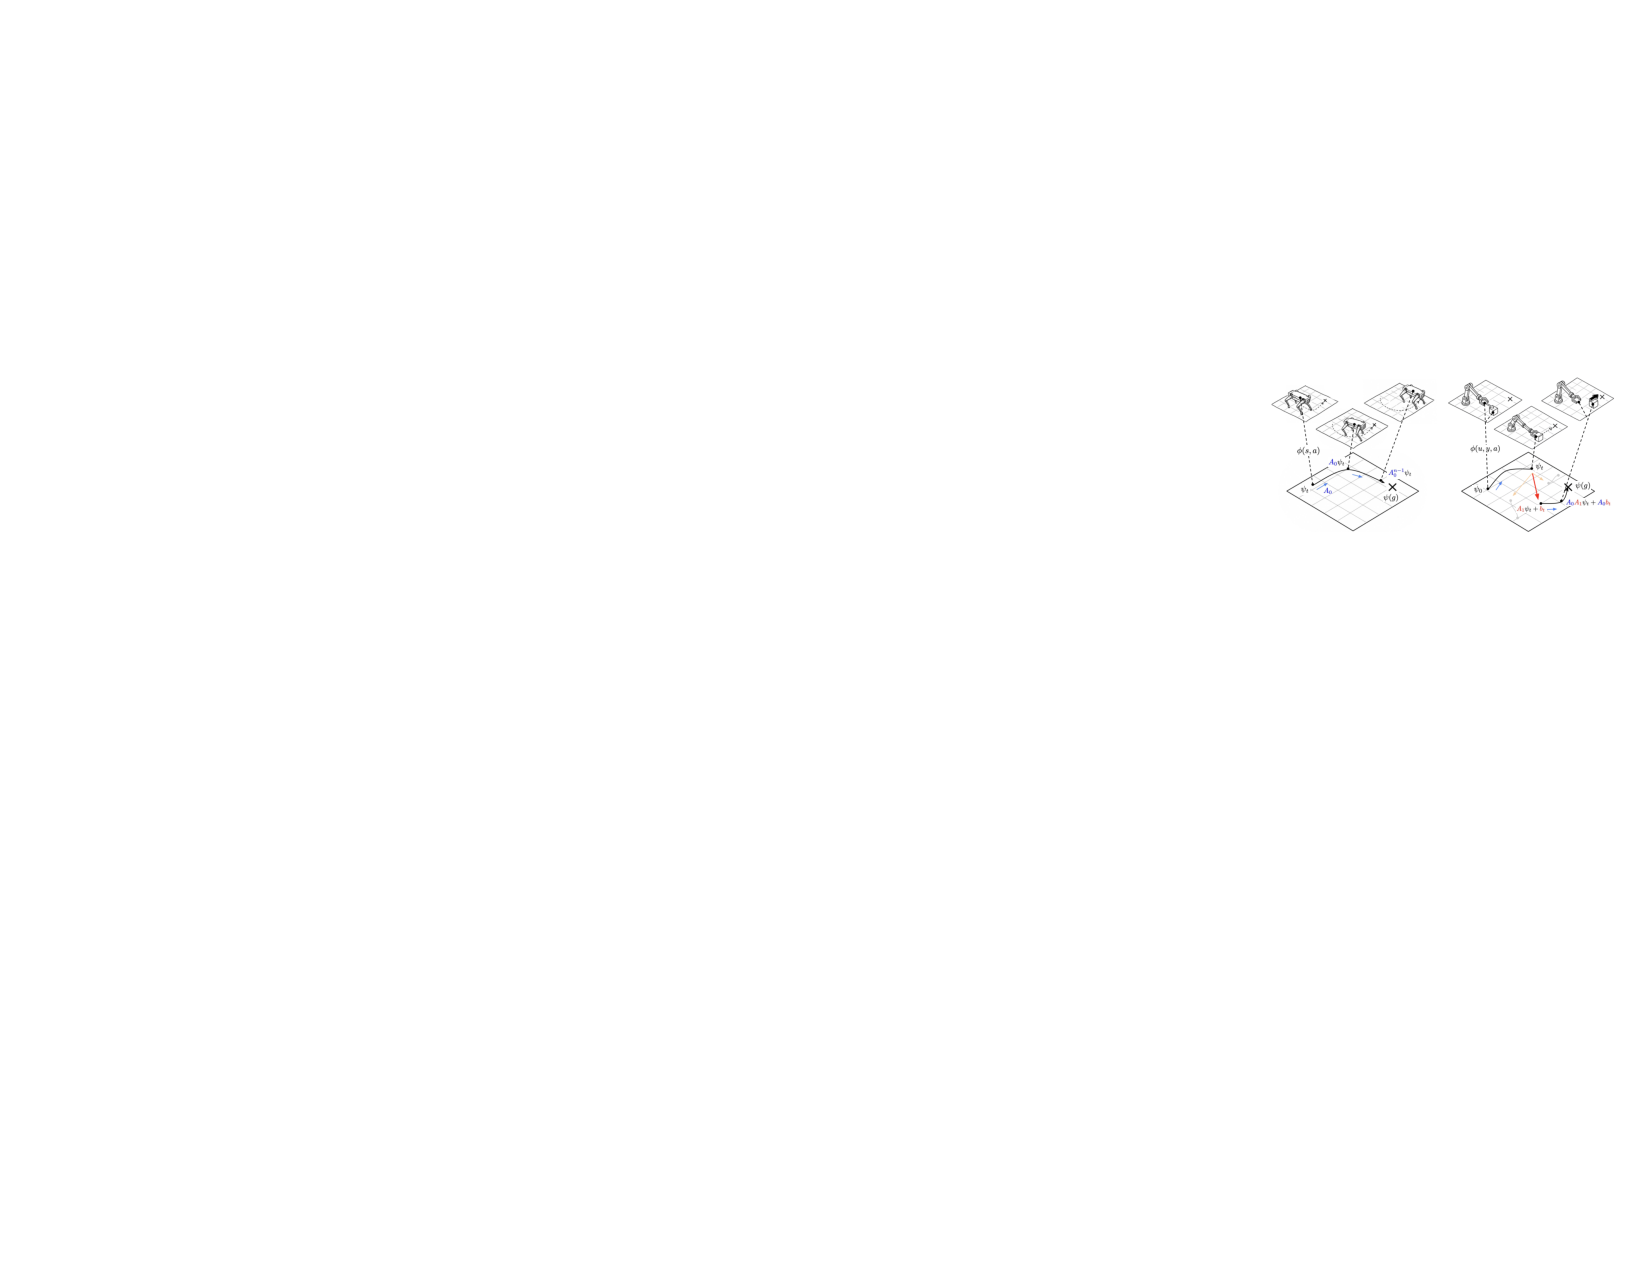
\includegraphics[width=0.98\textwidth]{figure/theory-illustration.pdf}
    \caption{
    Theory illustration.
    }
\label{fig:theory_illustration}
    \vspace{-1em}
\end{figure}

Proposition~\ref{prop:energy-perturbation-appendix} shows that endpoint CRL can produce fragile interaction energies for two reasons. First, the bridge shift itself may be estimated inaccurately when few samples directly cover the interaction. Second, even a small bridge error is propagated through $A_0^k$ before it supervises the endpoint energy. Thus, the endpoint energy error depends jointly on the local bridge error $\|e_{\tau}\|$ and the propagation factor $\|\Sigma_k^{-1/2}A_0^k\|$.

This explains why interaction-centered sampling is useful. Samples close to the bridge have smaller $k$, so the bridge shift is observed with less propagation. Increasing the number of such samples also improves the local estimate of $\delta_{\tau}$. Therefore, Interaction-Weighted Resampling targets both terms in the bound: it reduces the bridge estimation error and shortens the propagation path through which that error affects the CRL energy.